%Sigma + Vile.tex
\chapter{Sigma}\label{char:Sigma}
\begin{figure}[h]
	\centering
	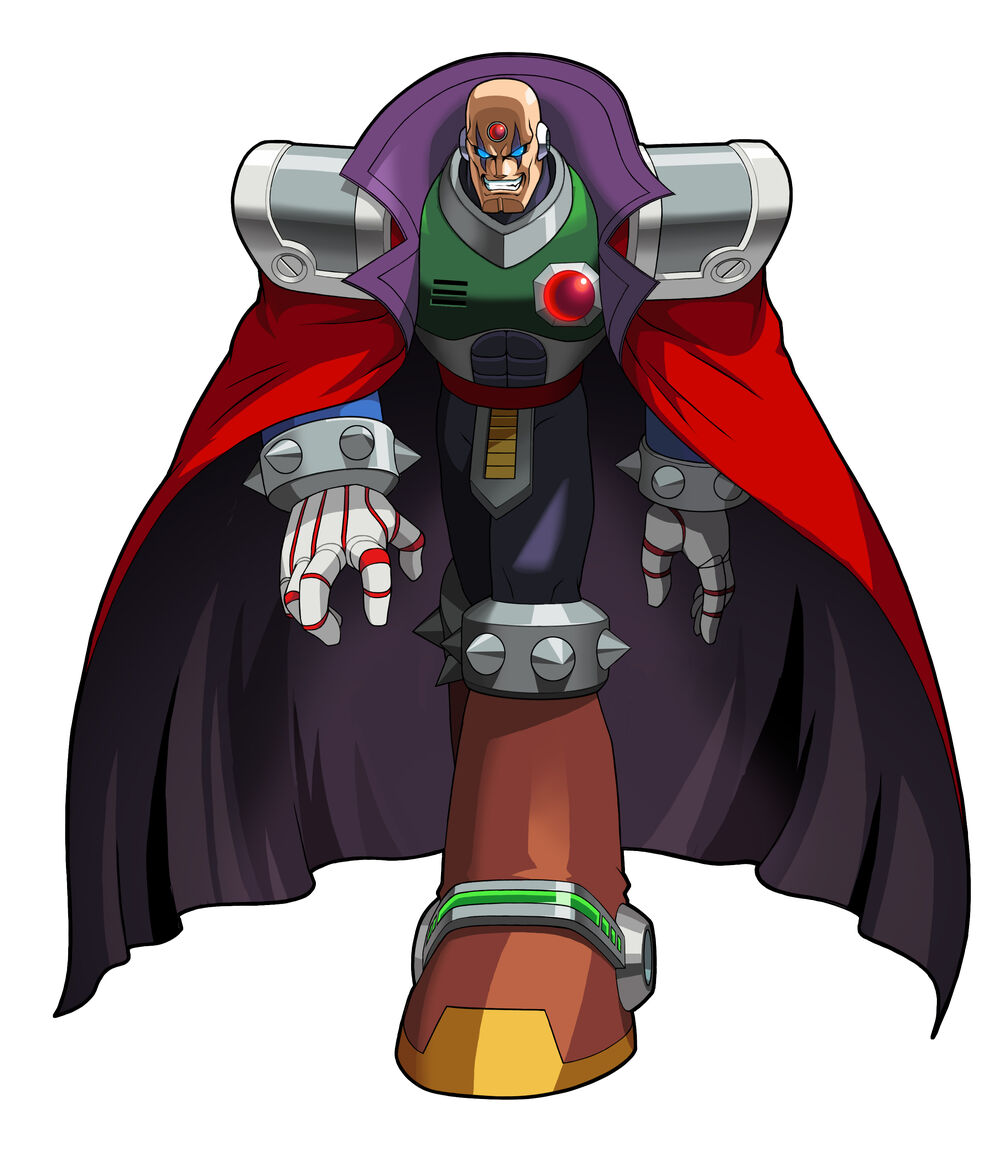
\includegraphics[width=0.4\linewidth]{figures/X1/Sigma_stages/MHXSigma.jpg}
\end{figure}
Sigma is Dr.~Cain's greatest creation. Developed to be a strong leader to face the Maverick threat, Sigma is equipped with latest design in term of brain circuit, which according do Cain himself should be fault-safe and prevent him from going maverick. Sadly things doesn't go as the Cain wished, as after solely two years of leading the Maverick Haunter Sigma not only goes maverick, but began a war against humanity bringing on his side a major part of Maverick Haunter which he led. To Sigma, in fact, humans are only an obstacle to reploids evolution, and should be eliminated to allow reploids to reach their full potential. 

In this chapter Sigma' action through the X series will be described. Since in the first game Sigma act only as the final boss, with very few interactions with X beside his boss quotes, for the first part of his story the description will stay closer to his \mhx version, as it gives more insight on Sigma's personality and motivations.

\section{Leader of the Maverick Haunters}
WIP. Information will be added at proper time.

\section{The X saga}
Sigma declares his war to humanity on July 4$^{th}$ 21XX, and launches an all-out attack onto Abel city, by deploying his troops to conquer strategical positions and assigning powerful reploids to protect them, but only after having first stroke the city  with a missile attack, as shown in \textit{Day of $\Sigma$}. In this occasion he has a first confrontation with X which Sigma easily defeats. However during the fight for a brief moment X manages to reach his full potential hitting Sigma and leaving his signature scars. After that he retires
into his fortress, waiting for his scheme to be completed. In truth, Sigma's plans not only aims at human extinction, but he also wants to discover X's true potential my forcing him to fight. To no surprise, in fact, X manages to defeat all his subordinate and, with the help of Zero, to infiltrate his fortress. Here Sigma prepare a last test for X, by resurrecting all defeated reploids and making them fight X once more\footnote{``\textit{Sigma must have brought his body back to life}''-X talking to a resurrected Launch Octopus-\cite{wiki:MM_MHX_script}}. X passes this trial too, even taking down Vile, and finally reaches Sigma which happily verify that he was right about X and reploids' unlimited potential, and than proceed to challenge him in a final fight, firmly believing to be superior. Sigma however misjudge X, which strikes him down even after he combines with a giant wolf-type mechaniloid (\ref{boss:wolf_sigma}) to further increase his power. Defeated in the body, but not in the spirit, Sigma's body sinks into the sea alongside his fortress while X, teleported outside, watches silently believing to have put an end to the war. Sadly, however, this couldn't be far from true, as in reality Sigma's true consciousness had already left his original body before the fight with X, preparing to resurrect again in case of defeat: ``\textit{What you defeated was not my true self. The machine that was destroyed was more like another body. I will materialize and resurrect once more}''~\cite{wordpress:X_japanese_script}.

\chapter{Vile}\label{char:Vile}
\begin{figure}[h]
	\centering
	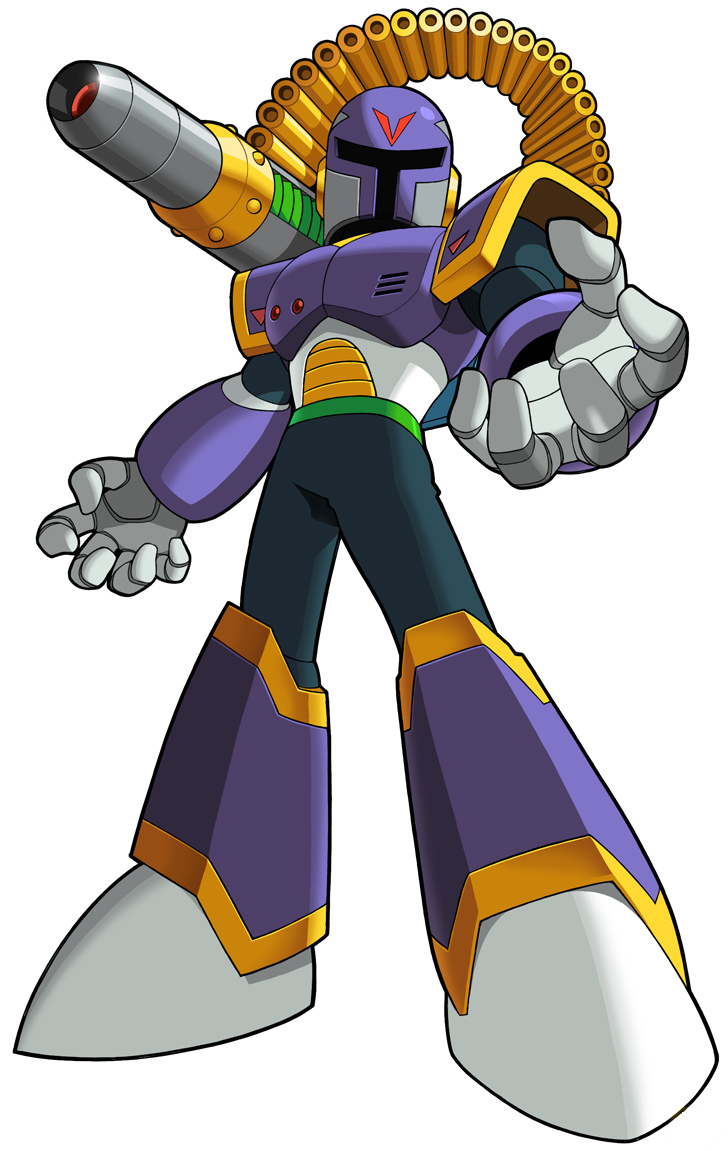
\includegraphics[width=0.3\linewidth]{figures/X1/Sigma_stages/MhxVile.png}	
\end{figure}

Although Vile does not play a major role in the X saga except for the first game, his status as recurring enemy in some games plus the presence of a dedicated game mode in the first game's remake, which better describe Vile's personality, are sufficient in order to dedicate this small chapter to him alone. 

Before beginning, however, it is important to appoint how differences between the original Mega Man X games and its remake Maverick Haunter X will be handled. In those games, in fact, Vile' personalty is slightly different, since in the former not many information are given beside his background and his dialogues as a boss, while in the latter, also thanks to his dedicated game mode, more details about his personality are given. In this document we will stick to the latter, as it incorporates almost every aspect of the original story too. Clearly it is debatable whether what shown in the Vile's mode is effectively true or not, as the game mode itself is presented as a what-if scenario and hence not canonical. However since this is the only source of additional information about Vile's personality, and for most part of the mode Vile's personality match with the real one shown in the effective game, what shown about Vile in Vile's mode will be used in the document and considered to be true.

Clearly what said until now regards only the first game of the series, as there aren't any remake for the other games Vile appears in.

\section{Before the war}
It is unknown when Vile was created or who build him. What is sure, however, is that Vile was designed purely for combat, as Zero points to X during their first meeting with him\footnote{``\textit{X, you shouldn't expect to defeat him, he is designed to be a war machine.}''- Zero}, maybe specifically to work as a Maverick Haunter. Thanks to his equipment, Vile quickly became one of the highest-ranked Maverick Haunter of the 17$^{th}$ elite unit (the same as X, Zero and Sigma), with the Special-A (SA) rank, the same as Zero and Sigma, despite his bad attitude. According to information given, in fact, Vile have always behave with arrogance and superiority, only taking orders from himself\footnote{``\textit{I'll tell you one thing$\dots$ I don't like working for others.}''-Vile~\cite{MHX:Vile_script}}, disrespecting superiors\footnote{``\textit{You don't respect authority. You don't follow orders. I pity you}''-Armored Armadillo~\cite{MHX:Vile_script}} and working alone, not having anyone to consider friends and, on the contrary, disliking some of his comrades\footnote{``I've always hated you, Storm Eagle. You and that smug face of yours''-Vile~\cite{MHX:Vile_script}}, especially X. Although this he still has the respect of his commilitones, such as Sting Chameleon (``\textit{It's Vile$\dots$ I used to have nothing but respect for you, you know.}''~\cite{MHX:Vile_script}).

It is with X, however, that Vile shows his worst. To him, in fact, X is only a weak reploid and nothing more, and thus he doesn't understand the reasons why people around him claim X to have incredible power. Because of this Vile develop a grudge and hatred for X, which in reality only cover his jealousy, and dedicates himself to the task of defeating and humiliating him for as much as he can, in order to prove himself and to others that he is the strongest reploids.

Vile's situation get worse when a fault in his electronic brain occurs. Due to this fault Vile starts to enjoy much more the pleasure of haunting and destroying his target, almost to the point of being an obsession, making him ignore any collateral damage he could cause with his actions and aggravating his position inside the Haunter organization up to the point of being considered to be a borderline maverick. This leads the high command  to preemptive arrest him, in waiting for a sentence on his destiny.

\section{Mega Man X}
Shortly before the beginning of the first game Vile is set free by a soon-to-be maverick Sigma, which asks for Vile help to defeat X as he fear X could interfere in his plans of changing the world\footnote{``I need your help, to defeat X [$\dots$] in order to ensure our future and speed along our evolution''-Sigma~\cite{MHX:Vile_script}}. Although Vile's hate for taking orders, the idea of defeating X is sufficient for him to follow Sigma and help him with his plan. In reality, however, Vile's claimed objective is to follow Sigma only until X's defeat and then to turn against Sigma himself, defeating him to change the world as he desires, as he says to X after battling with him on the highway (``\textit{There's nothing you can do! I'll defeat you and Sigma! Then I'll change the world!}''~\cite{wiki:MM_MHX_script}). In this situation, however, Zero comes and save X, damaging Vile's armor and forcing him to retreat (showing also that, despite his obsession, Vile still retains a tactical mind). 

It is unknown what Vile does during most part of the X game, as he only appears later, at the beginning of Sigma fortress. An hypothesis that could be  formulated is that in the meanwhile Vile had worked and upgraded his ride-armor, as during his last encounter he uses a different, customized version of it, and setting up a trap to prevent Zero from stopping him again. This, however, are only hypothesis without any confirmations.

Vile's final appearance is inside Sigma Fortress, where he attempts again to destroy X, this time capturing Zero first. He almost succeeds in doing it, but he underestimate Zero and X's potential as the first breaks free and destroy his armor, by sacrificing himself, and the latter takes him down. The same fate waits Vile in his own game mode, but with the addition of a final dialogue between a dying Vile and Sigma. Here Vile's true intentions are finally revealed: he's solely purpose in life has always been defeating X and nothing more, as everything he claimed were only justifications for his actions. In fact, Vile has never had any idea of what to do had he managed to beat X:
\begin{quote}
	SIGMA: What exactly did you plan to do, Vile? Would you stand before me as a Maverick Hunter? Kneel before me and place yourself at my mercy?
	
	VILE: ...What did I.. plan to do? Heh... thinking about it now, I'm not actually sure

	[$\dots$]

	VILE: I don't care what happens to this world... By defeating X\footnote{In Vile's game mode he manages to take down both Zero and X, only to be destroyed because of a surpise attack from Zero, immobilize him and gives X the time to hit him. Hence the reason why Vile claims to have defeaten X}, I've validated
	my own existence... and that's all that matters to me now.
\end{quote}
